\documentclass{article}
\usepackage[utf8]{inputenc}
\usepackage{caption}
\usepackage{amsmath}
\usepackage{amssymb}
\usepackage{mathtools}
\usepackage{multicol}
\usepackage{graphicx}
\usepackage{wrapfig}
\usepackage{float}
\usepackage[makeroom]{cancel}
\usepackage{mhchem}

\graphicspath{ {../images/} }

\renewcommand{\baselinestretch}{1.5} % line spacing
\newcommand{\fline}{\par\noindent\rule{\textwidth}{0.1pt}} % horizontal line (wide)

\title{Unit 2 Kinetics\\Collision Theory}
\author{Peter Zhang}

\begin{document}

\maketitle
\newpage
\tableofcontents
\newpage


% lesson 1
\section{Collision Theory}

\subsection{Rate}
Rate is defined as concentration over time. It is anything that you can observe/measure as time changes

%insert image
\fbox{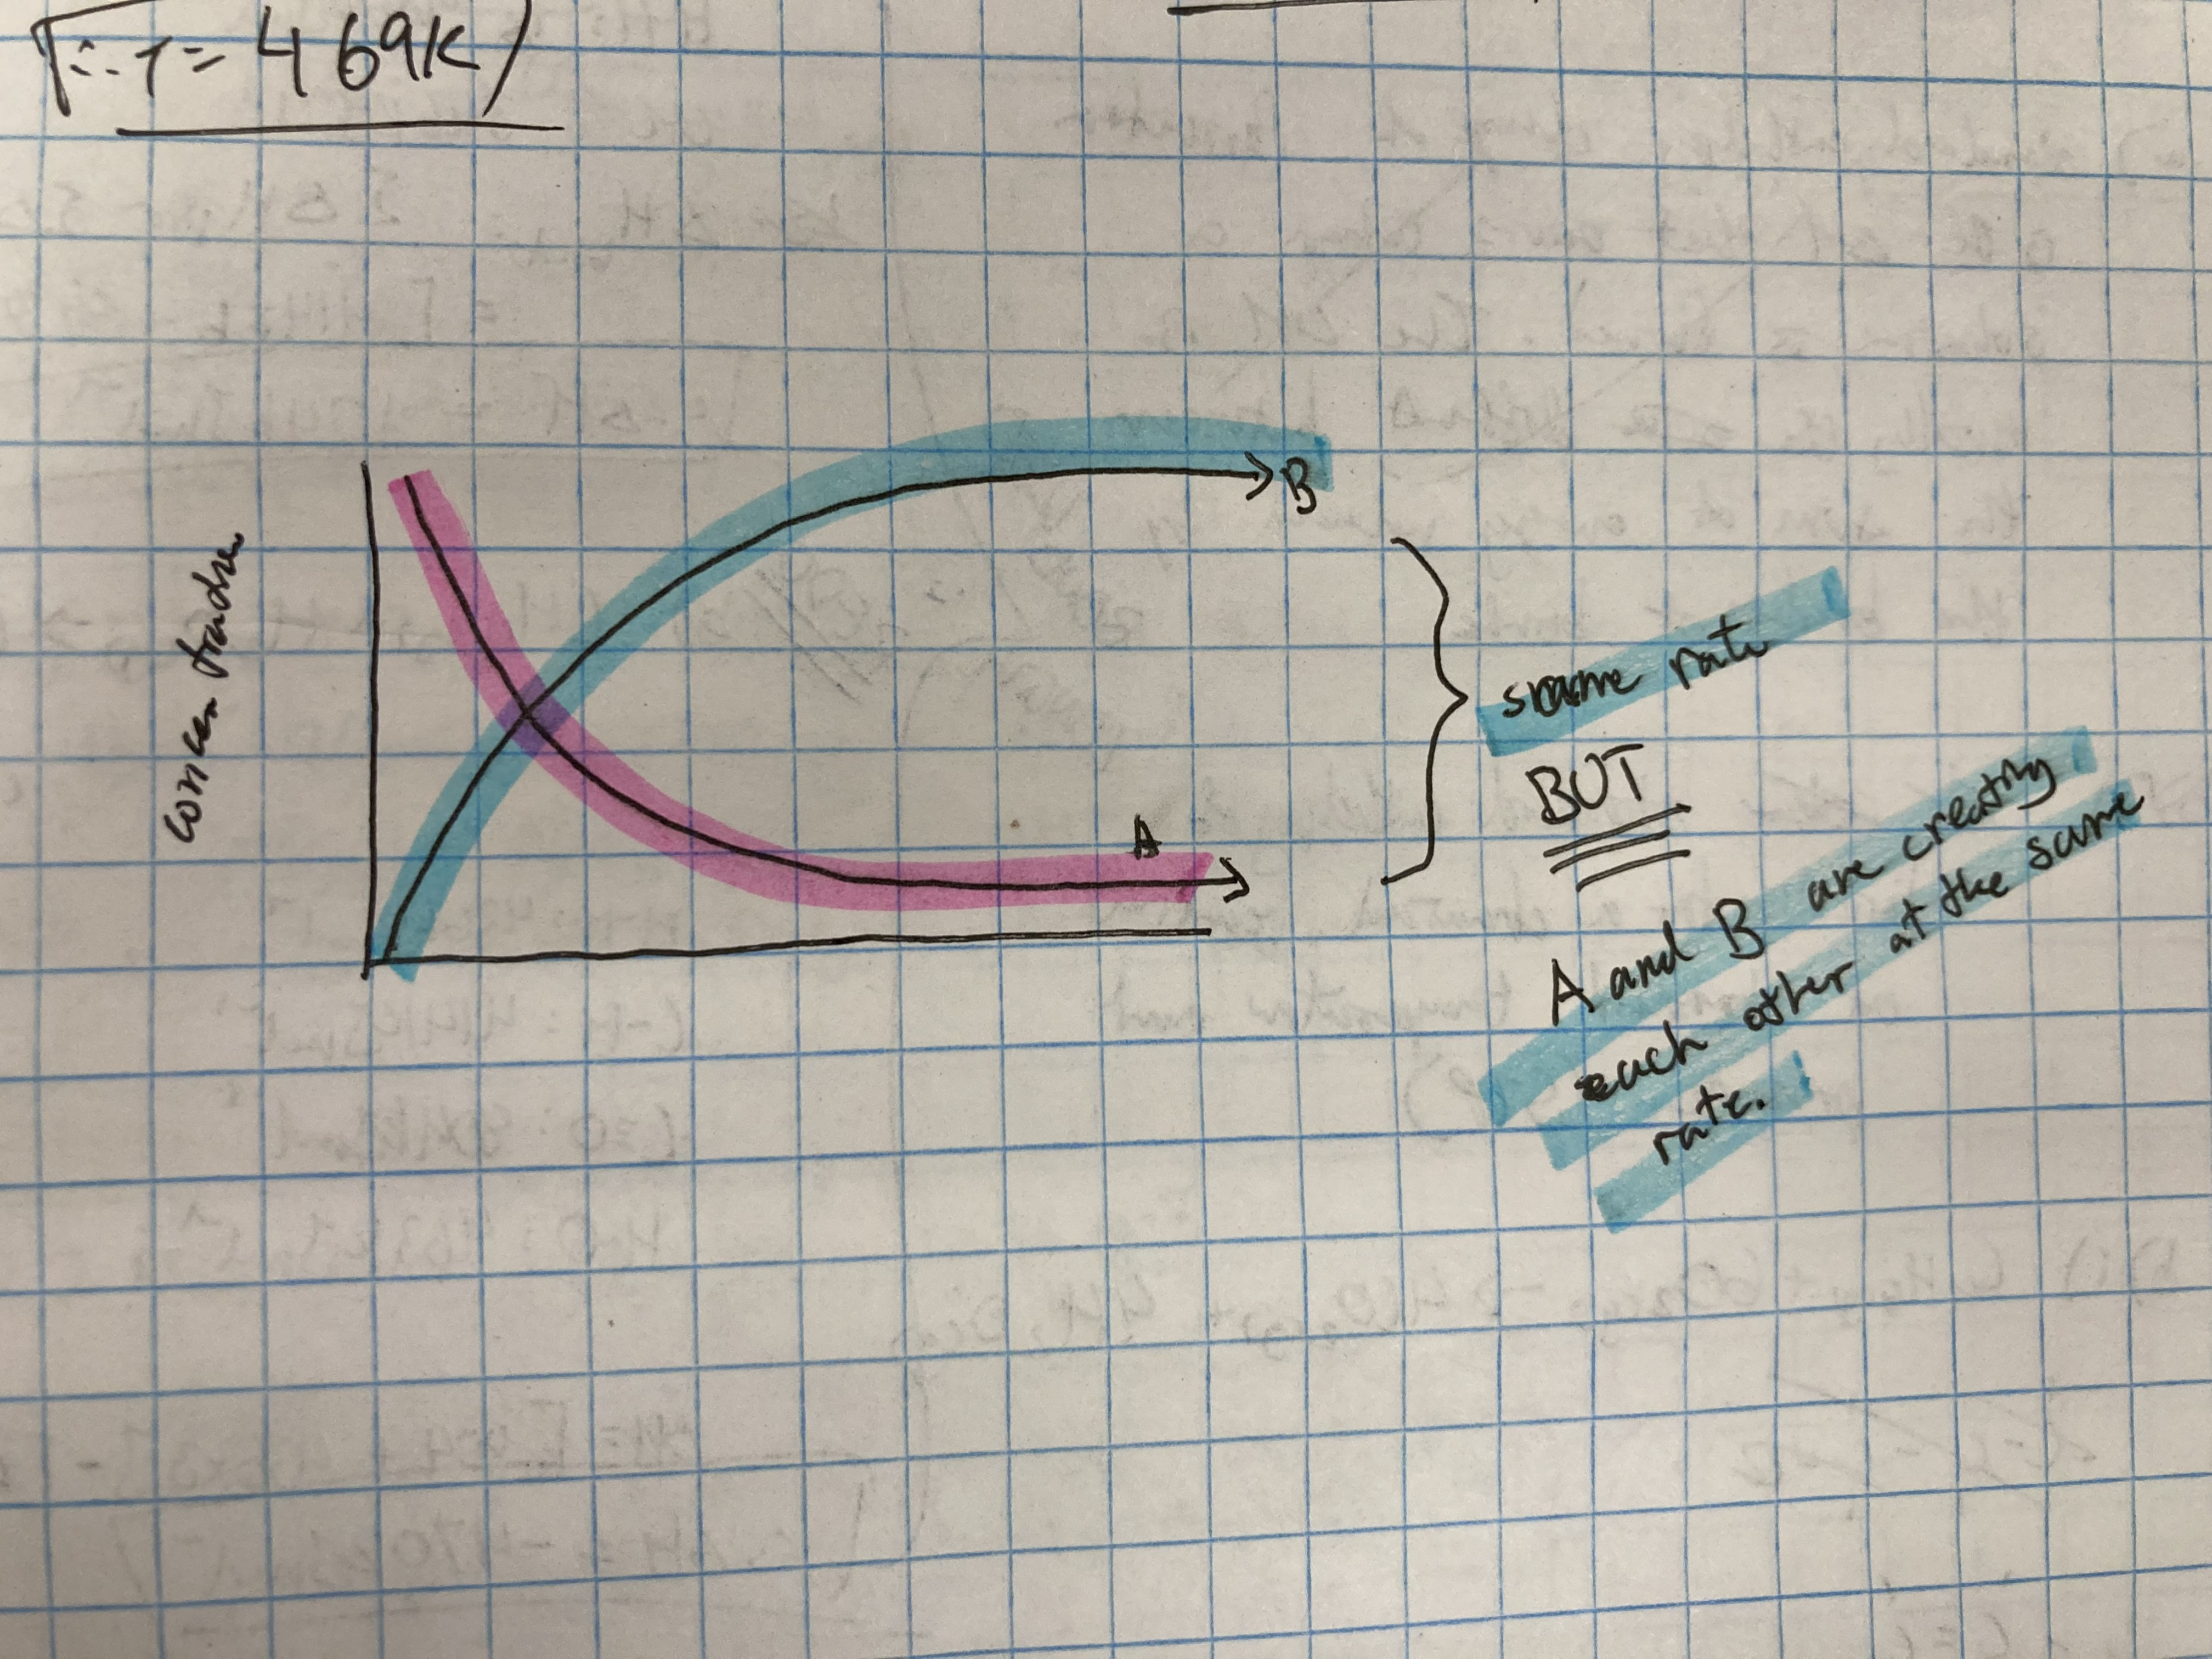
\includegraphics[width=\textwidth]{2.1fig1.jpg}}\\

\ce{A <=> B}

Other ways to measure rate:
\begin{itemize}
\item change in volume of gas
\item change in mass
\item change in transmission of light (very few reactions but \textbf{change in color (not light)}
\item change in [] for titrations
\item change in [] using conductivity
\end{itemize}

Time can either be a constant variable or something that changes...


$$rate: \frac{-\triangle{[reactant]}}{\triangle{t}}$$

$$rate: \frac{\triangle{[produce]}}{\triangle{t}}$$


\subsection{Units for Rate}
Rate is measured in $mol/dm^{3}time^{-1}$


\subsection{Questions}
\subsubsection{Question 1}
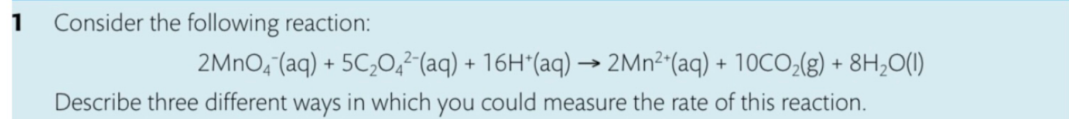
\includegraphics[width=\textwidth]{2.1fig2.png}

3 ways to measure rate of this reaction
\begin{itemize}
\item change in color (because change in oxidation state)
\item gas production (gas is produced from fully aq solution)
\item conductivity (concentration of ions changes)
\item change in pH (\textbf{\ce{h+}} are used up)
\item change in volume (of water b/c the water volume should \ce{v} as gas escapes)
\end{itemize}


\subsubsection{Question 3}
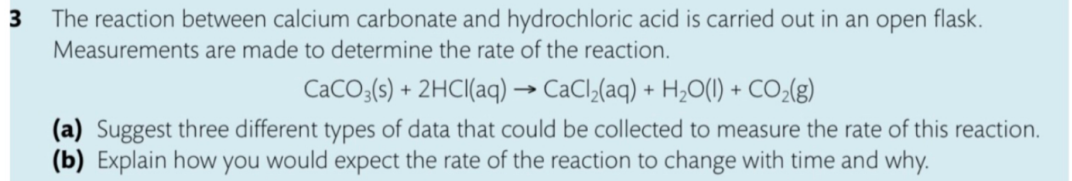
\includegraphics[width=\textwidth]{2.1fig3.png}

Part a:
\begin{itemize}
\item change in volume/gas (the volume changes as gas escapes)
\item change in pH (HCl breaks down into H2O)
\item change in mass (solid reactant/change in values of ligand and gas escapes)
\end{itemize}

Part b not answered.

\subsection{Collision Theory}
Particles move with random motion/energy $\rightarrow$ the energy is \textbf{Kinetic energy}.

There is so much more going on with particles that we cannot predict anything to 100\%.
\begin{itemize}
\item Even particels within a molecule can have different energies\\ 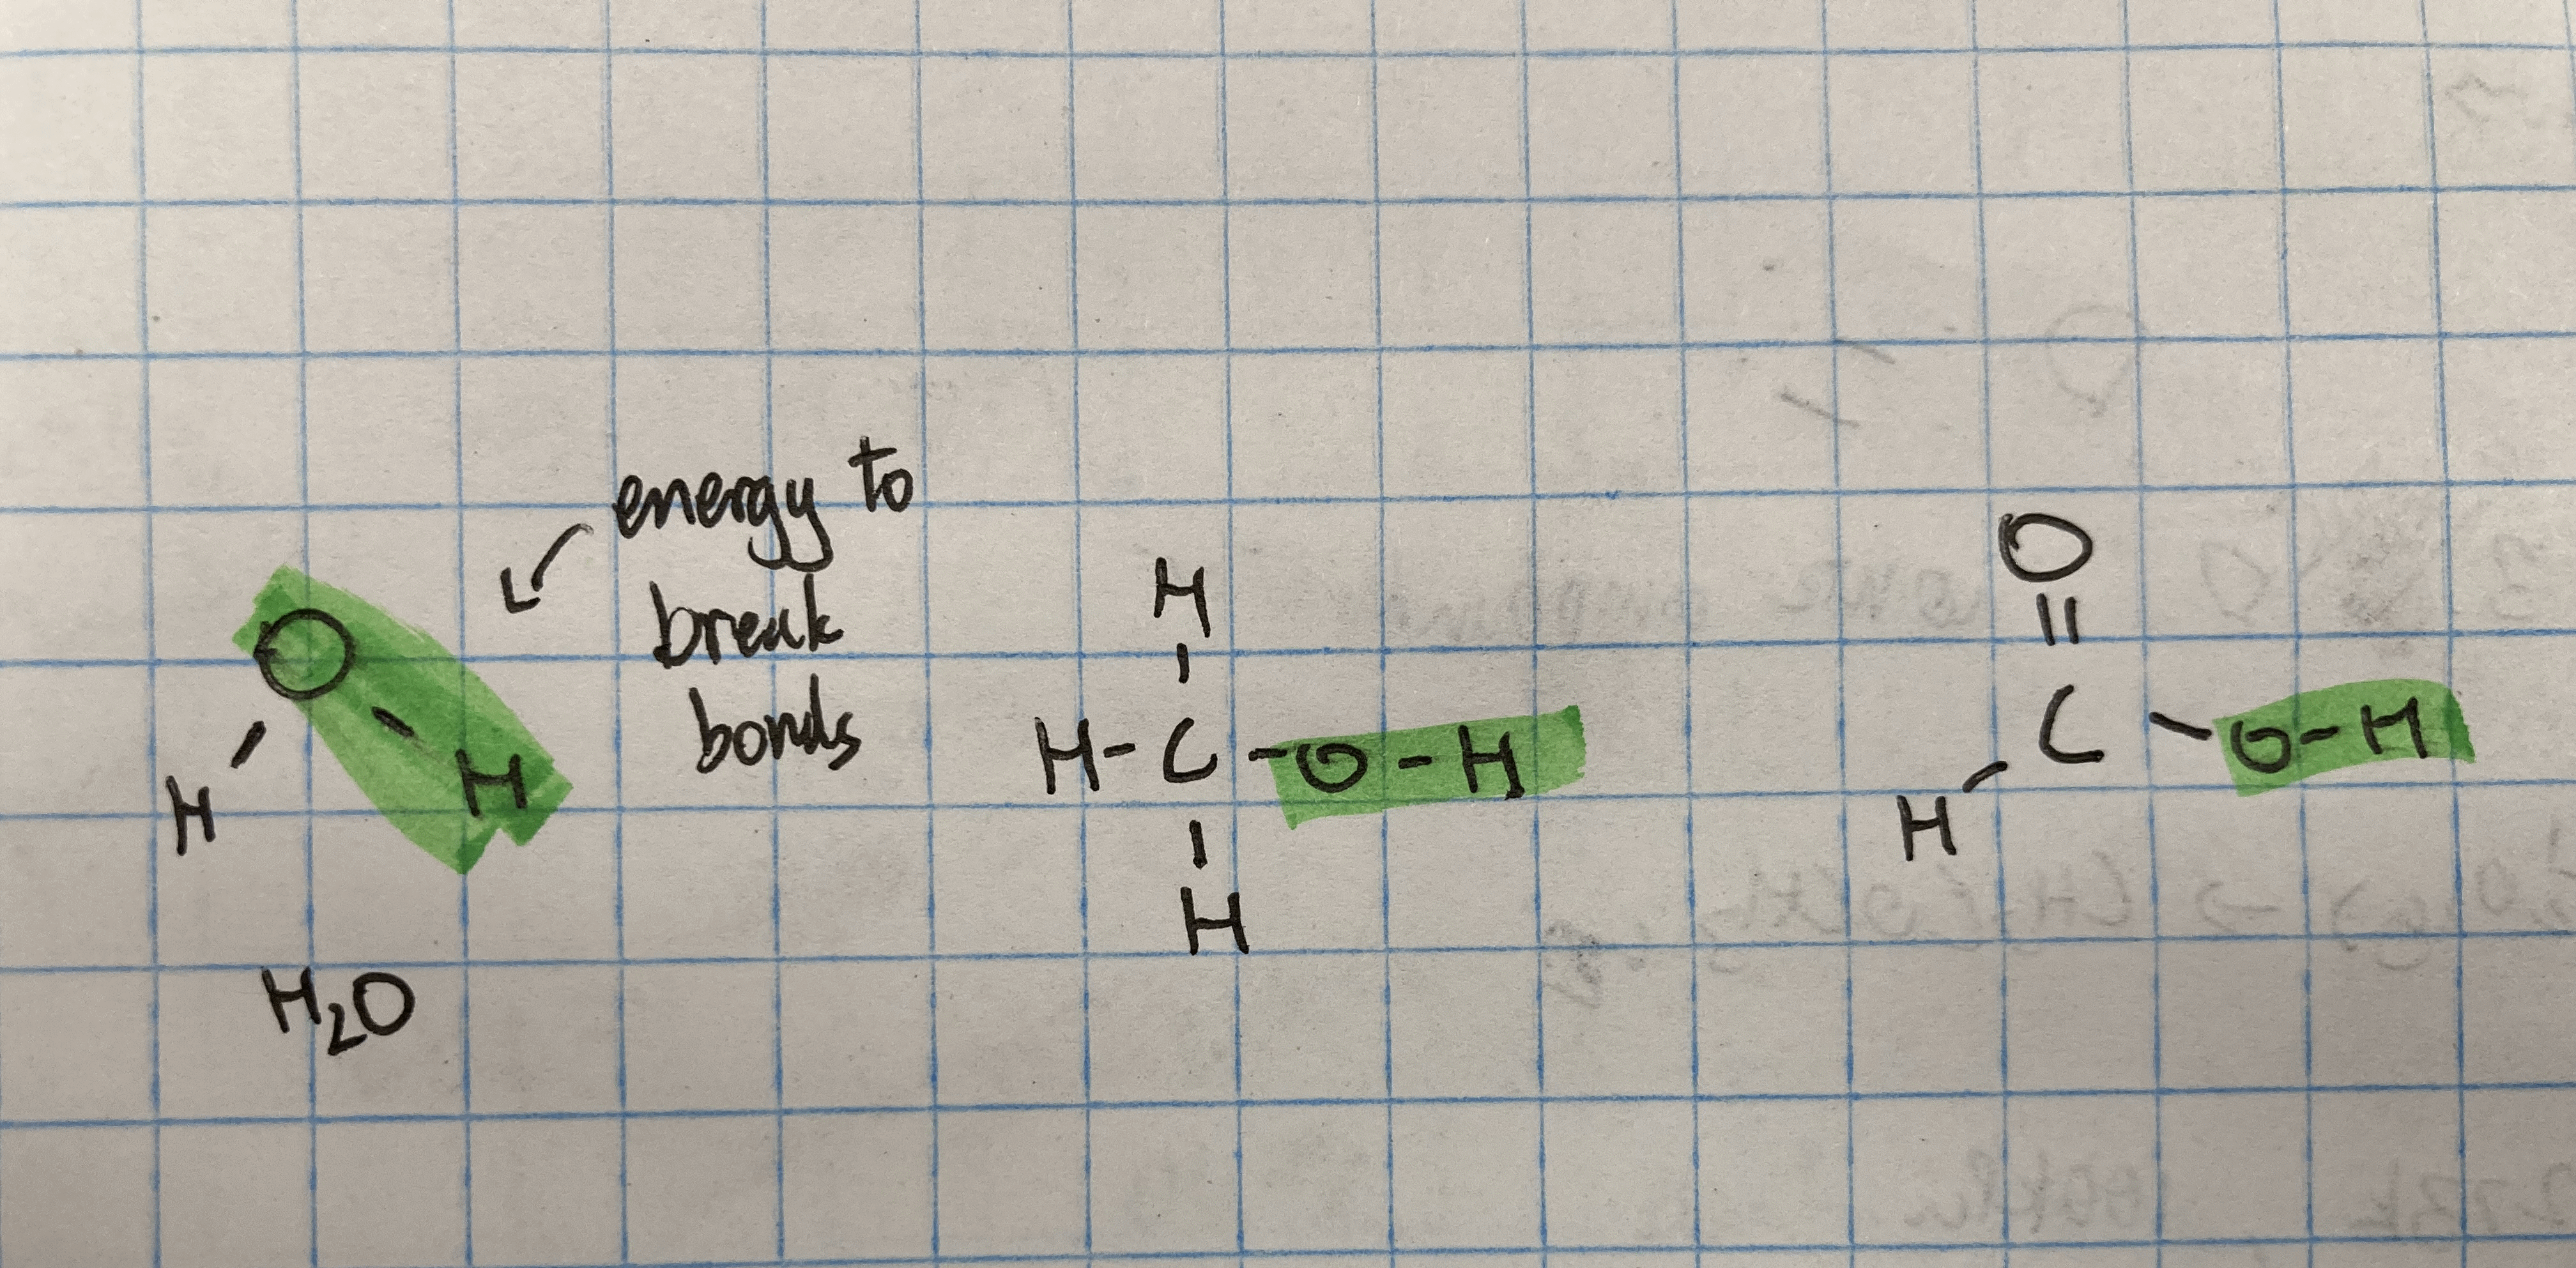
\includegraphics[width=\textwidth]{1.3fig1.png}
\item Rate is dependent on \underline{successful} collisions\\Every single molecule is hitting each other but this does not mean that all of them are creating new compounds. \textbf{Not all particles interact}.Just hitting something does not results in successful collision. 
\end{itemize}

\pagebreak

\subsubsection{Factors | Energy/Activation Energy}
\begin{itemize}
\item	\begin{itemize}
		\item Energy - requires a minimum energy to be reached
		\item Known as \textbf{activation energy} given symbol \textbf{$E_{a}$}
		\item Energy needed to \textbf{overcome repulsion} between atoms
	\end{itemize}
\item Activation Energy
	\begin{figure}[H]
	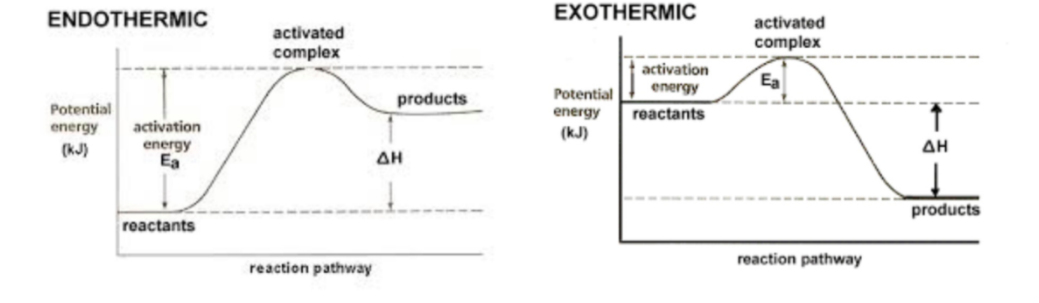
\includegraphics[width=\textwidth]{2.1fig4.png}
	\end{figure}
	\begin{itemize}
		\item a bunch of random things can exist before a final product is created
		\item \ce{HCl_{aq} + NaOH_{aq} $\rightarrow$ H+ + O- + Na+ + OH- $\rightarrow$ HClNaOhHC(Na)H_2O $\rightarrow$ NaCl + H_2O}
	\end{itemize}
\end{itemize}

\subsubsection{Factors | Geometry}
Lets say the energy required is reached... We also need to make sure that the geometry of the collision is correct. Incorrect types of geometry will result in no reaction.

\begin{figure}[H]
	\centering
	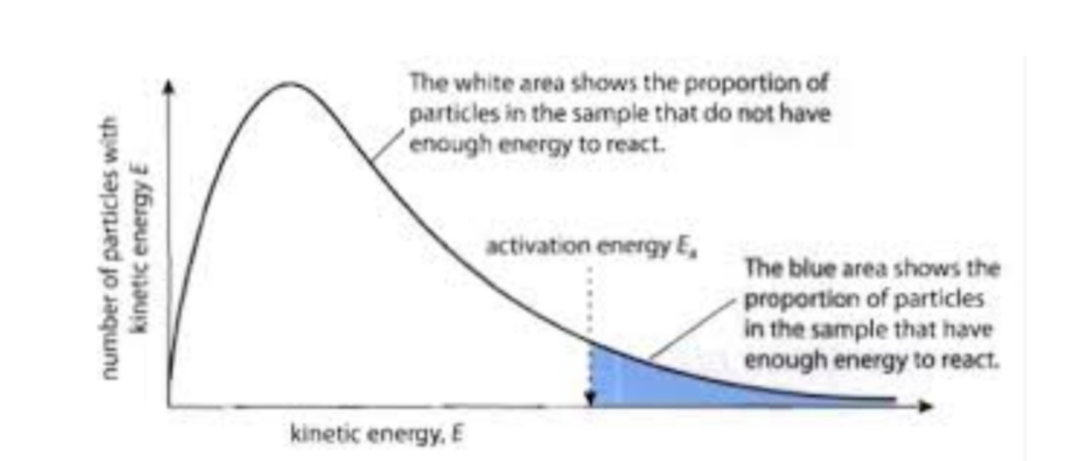
\includegraphics[width=\textwidth]{2.1fig5.png}
	\captionof{figure}{Maxwell Boltzmann Diagram}
\end{figure}

The maxwell botlzmann diagram tells us the kinetic energy of a system? (google this please)















\end{document}